
\section{Average segregation time}\label{sec:aveseg}
As mentioned in the introduction, the segregation time at \(n\%\) is defined as the number of generations until at least \(n\%\) of the population on a board lives in homogenous groups. 
Where person \(i\) is said to live homogenous if for any neighbour \(j\) of \(i\), we have \(\text{Type}(j)=\text{Type}(i)\).
This gives immediate rise to questions concerning the relation between the choice of \(n\) and the average segregation time at \(n\%\). 
Furthermore, it is unclear if segregation at \(n\%\) is guaranteed before a board reaches an equilibrium and what the effect is of the happiness boundary on the existence of a segregation time.\\

To research any of the given questions, we will first have to formalise our choices of board as well as the questions proposed.\\


\subsection{Formalisations}
Prior to starting any test or properly formalising our research questions however, we note that segratation at \(n\%\) does not necessarily have to happen: 
If we consider \(n=100\) on the standard board with happiness \(1/3\). We will nearly never have total segregation before the board reaches an equilibrium.
Therefore one might instead consider the average fraction of segregation at equilibrium,for any given happiness fraction. \\

Furthermore, the average segregation time as function of the segregation fraction should theoretically be a strictly increasing function since for any given board we have:
\begin{align*}
&n\% \text{ lives in homogenous groups after } k \text{ generations } \Rightarrow\\
& m\% \text{ lives in homogenous groups after } k \text{ generations, for any } 0 \leq m \leq n
\end{align*} 
Having noted these facts, we can now properly formalise the research questions.\\
The following questions are proposed:
\begin{enumerate}
 \item What is the relation between the average segregation time and \(n\).
 \item What is the average segregated fraction of the population after a board reaches equilibrium for given choices of happiness.
 \item For any Happiness Rule ranging from 0 to 1, how often do we reach at least $60\%$, at least $80\%$ or even full ($100\%$) segregation?
 \item For $60\%$ and $80\%$ segregation, what distribution do we get for the segregation time, if $HR = 1$? Are these comparable?
\end{enumerate}

To establish results regarding these questions, we consider different setups in testings. We will be testing two different boards.
The first board to be analysed is the standard board. The second board is a larger 
"4-Type" board. The details are specified below:
\begin{table}[h!]
\centering
\caption{Specs of the two considered boards}
\label{my-label}
\begin{tabular}{l|l|l}
  & Standard Board & 4-Type Board\\ \hline
Number of types:& 2 & 4 \\ 
 Length:& 8 & 10  \\
 Width:& 8 & 10  \\
 Happiness:& 1 & 1  \\
Population per type: & 20 & 16  
\end{tabular}
\end{table}
\\
The 4-Type board is constructed to maintain the same ratio of inhabited and uninhabited spots as the standard board. The choice of happiness on these boards is 1 unlike the usual \(\frac{1}{3}\). 
This guarantees that for any \(n\leq 100\), segregation at \(n\%\) takes place prior to the board reaching an equilibrium. 
To observe the average segregation time \(n\%\) for any \(n\), 500 simulations will be ran per board and averaged out in order to give an approximation for the average segregation time at \(n\%\).
Likewise the average segregated fraction will be estimate by the average of the segregated fraction of an equilibrium from 500 simulations with given happiness \(q\).
\subsection{Results}
\subsubsection{Question 1}
The results regarding the first question are shown below:\\
\begin{figure}[H]
    \centering
    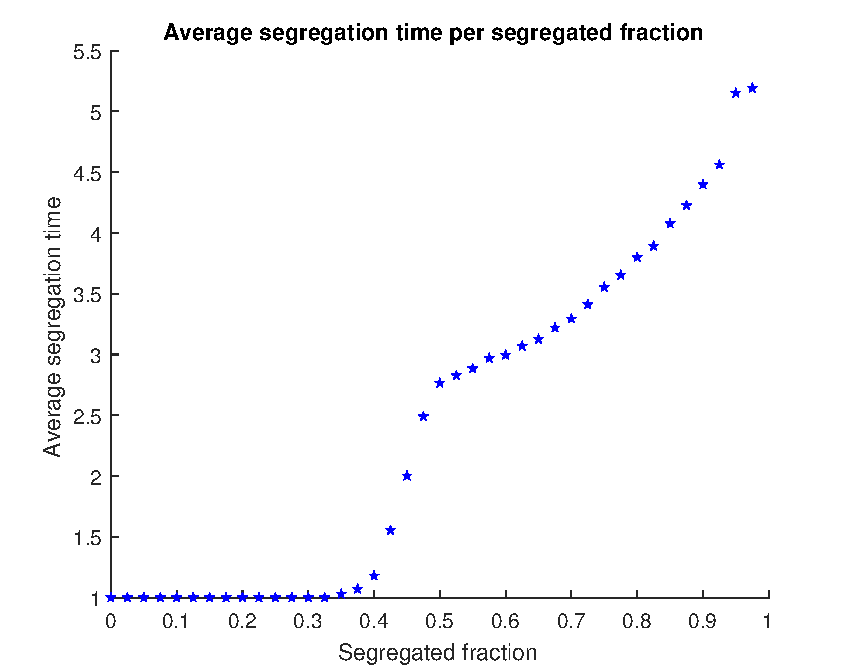
\includegraphics[width=0.8\textwidth]{aveseg_sb_2}
    \caption{Average segregation time on the standard board}
    \label{fig:avesegsb}
\end{figure}

Most notable of figure \ref{fig:avesegsb} is that it is neither linear nor exponential, which is what one might initially expect. Instead, it appears to be partially exponential and partially lineair. From the figure, we note that the average segregation time increases fastest between 0.4 and 0.5. 
Which is to say that it takes three times longer for 50\% of the population to live in homogenous groups than for 40\%.
Also note that the 'lift off' is approximately at $\frac{1}{3}$, but it is unlikely that this has anything to do with the standard happiness rule of $\frac{1}{3}$.\\

\textbf{Partial explanation} \\
The first part of this graph is easilyunderstood. 
When the board is initially formed, the odds are fairly high that several persons might already live homogenous, Due to the HR of 1, any non homgenous person will move, resulting in a further segregation. As the boundary of \(10\%\) is fairly low, it is likely that this will be achieved in less than 1 generation. 
The second interesting segment of this graph is the segment between 0.4 and 0.5, as mentioned, the figure shows that it takes considerably longer to reach a segregation of \(50\%\) than it takes to reach \(40\%\). 
This can be argued from a sociological perspective as follows some people are in general unhappy with their lives and will thus move to a new location anyways, the process of segregation, is a fairly lenghty process this way. However once people discover that their close neighbours are moving, they in turn decide to move as well. 
This does not neccessarily result in more moves, however as one type leaves, the other type is to remain in place, since they will tend to be more homogenous when their opposite type leaves.
Thus once 50$\%$ segregation has been reached, it becomes easier to segregate even further. Since the repositioning of one individual may result in three people becoming homogenous. This explains the part between $50\%$ and $70\%$. It might appear reasonable to believe that this increase will continue and that it that it would take at most two more generations to reach equilibrium but after $70\%$ segregation, it becomes harder for individuals to move to a homgenous location.
 This is also heavliy impacted by the laws defined in the model, a person will not move to the best location but to the closest better location, which might lead to a person moving from one disfavourable location to another. \\

Next, we consider the same question however this time on the 4-Type board. This gives  following results:


 \begin{figure}[H]
    \centering
    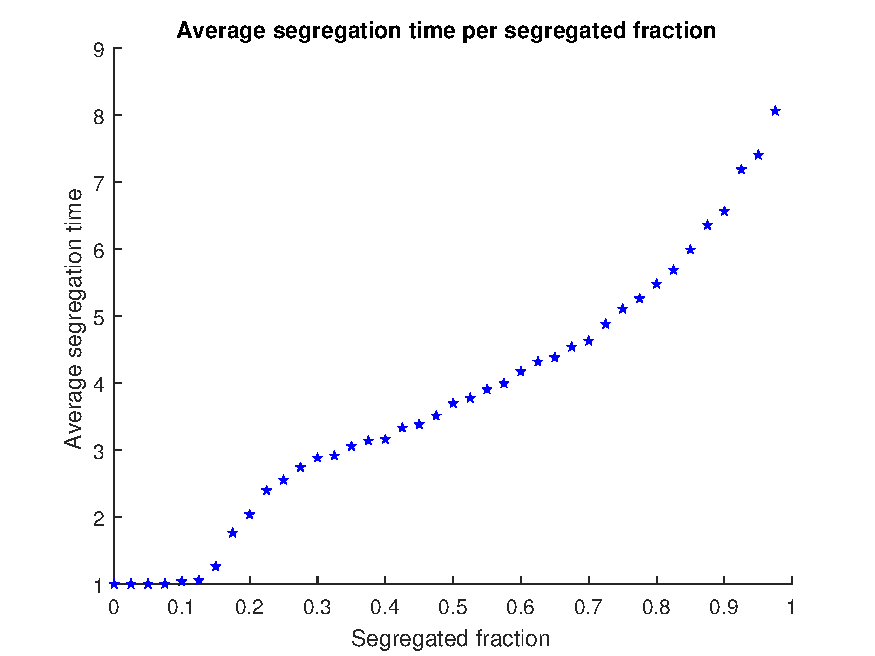
\includegraphics[width=0.8\textwidth]{aveseg_4b_2}
    \caption{Average segregation time on the 4-Type board}
    \label{fig:aveseg4b}
\end{figure}

The most notable difference between this figure and the figure \ref{fig:avesegsb} is that the 'lift off' lies happens much earlier than in figure \ref{fig:avesegsb}. 
Although this difference feels intuitive, we will give a formal explanation. 
Consider the probability that any individual $i$ has $a$ neighbours of the same type, and no neighbours of another type, given $k-a$ empty spots, where $k$ is the maximum number of possible neighbours for the location of $i$. 
In the basic model, this probability equals
\[
p_b = \frac{19}{39}\frac{18}{38}...\frac{19-a}{39-a} = \frac{\frac{19!}{(19-a)!}}{\frac{39!}{(39-a)!}} = \frac{19!(39-a)!}{39!(19-a)!}
\]
In the 4-Type model, this probability is
\[
p_4 = \frac{15!(63-a)!}{63!(15-a)!}
\]
which is less than half of $p_b$.\\

Also note that an individual is more likely to be homogenous if he/she is placed in a corner or on an edge. 
This is because a corner or edge spot has less possible neighbours than an interior spot, thus increasing the probability of only having neighbours of the same type. 
The 4-Type board has relatively more interior locations and fewer edge positions than the standard board. This effect also decreases the fraction of segregation prior to displacement of individuals.
However the people/boardspace ratio is maintained in both models and thus should not have too much of an impact on the results.\\

Another effect is the rise of the number of generations, that is, the time it takes before the board reaches full segregation. 
However, this effect is less strong than one might initially expect. 
On the standard board, it takes on average $5.5$ generations to reach full segregation. On the 4-Type board however, it takes $8.5$.\\

The remaining part of figure \ref{fig:aveseg4b} is quite similar to figure \ref{fig:avesegsb}: quick rise, followed by a slightly decreasing ascending relation. 
The explanation is similar to that of the basic model.
\subsubsection{Question 2}
\begin{figure}[H]
    \centering
    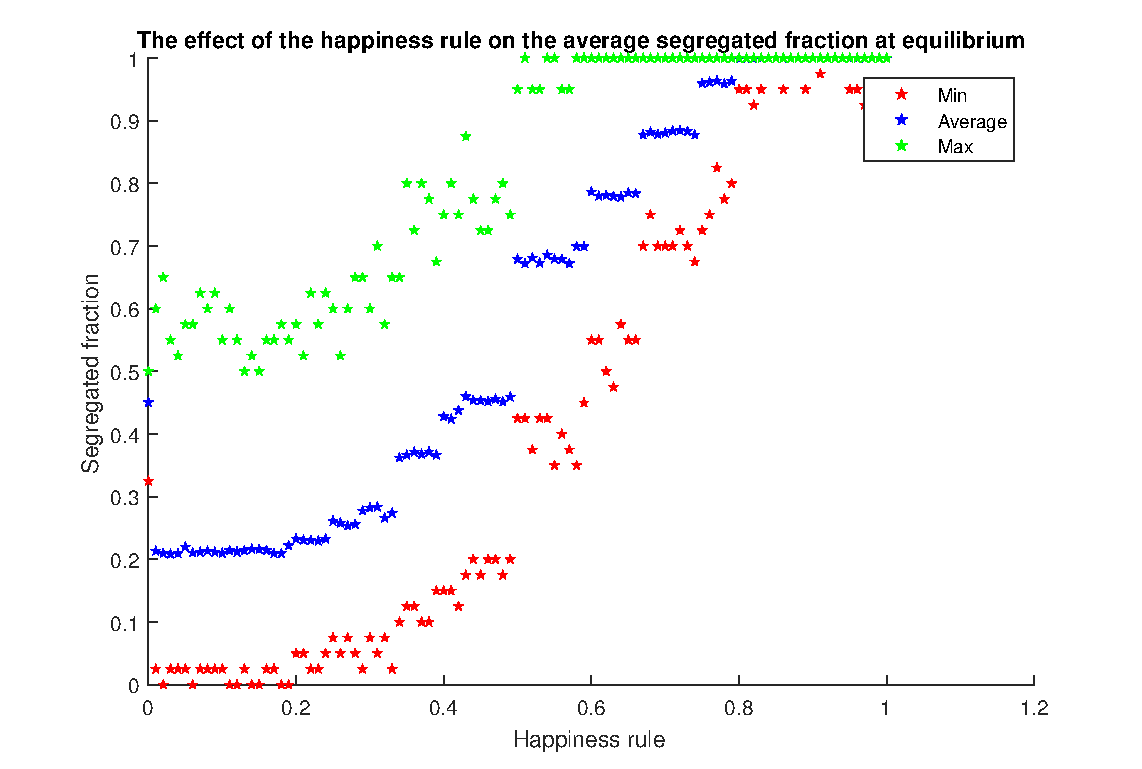
\includegraphics[width=0.8\textwidth]{habysegfrac_sb_2}
    \caption{Average segregated fraction as a result of happiness on the standard board}
    \label{fig:happysegsb}
\end{figure}

Figure \ref{fig:happysegsb} displays three scattered values. 
The red and green dots represent the minimum and maximum segregrated fraction of 500 boards for the given happiness. 
Notable in this picture is that the average segregated value is greater than the happiness. 
Another thing worth noting is that the segregated fractions tend to appear in different groups seperated by relatively large percentages.

\begin{figure}[H]
    \centering
    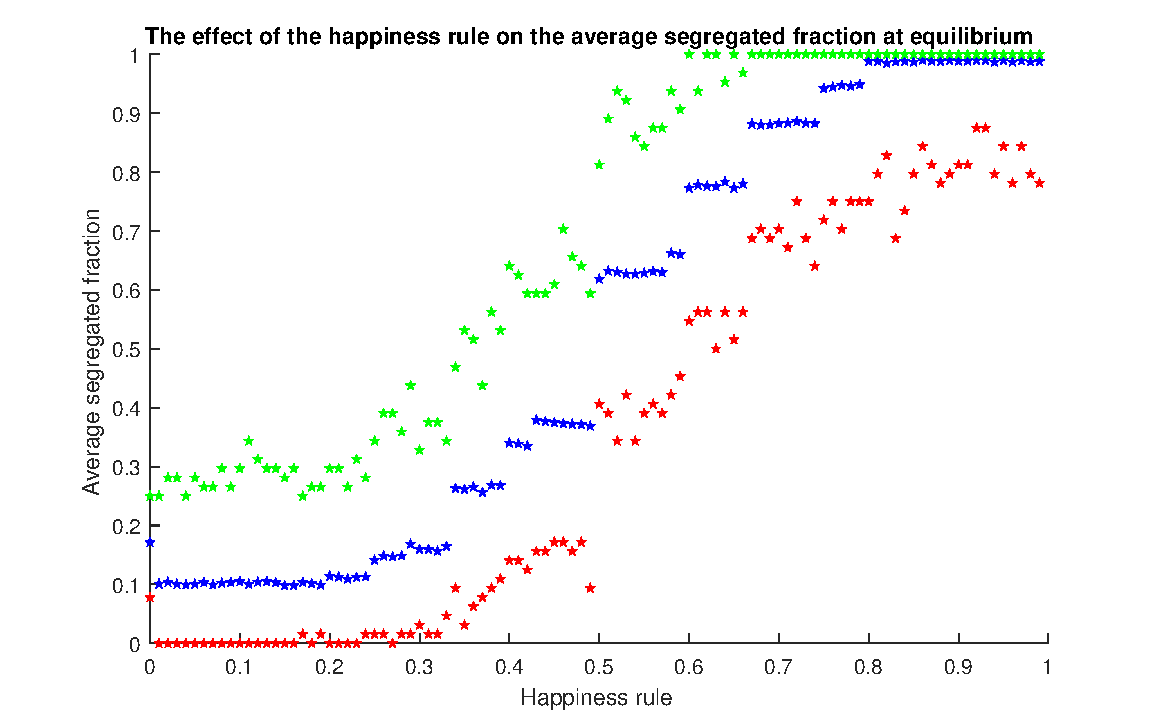
\includegraphics[width=0.8\textwidth]{habysegfrac_4b_2}
    \caption{Average (blue) segregated fraction as a result of happiness on the 4-Type board. Also included max (green) and min (red).}
    \label{fig:happyseg4b}
\end{figure}

Figure \ref{fig:happyseg4b} shows that contrast to the standard board, this board does not respect the property that the average segregated fraction is always greater than or equal to the happiness. 
A thing of interest however, is that the averages of both figure \ref{fig:happysegsb} and \ref{fig:happyseg4b} seem to cluster. 
This is because, as mentioned earlier, the effect of the Happiness Rule is quite discrete when using second order neighbourhood.

\subsubsection{Question 3}
In order to answer the third question, we ran 500 simulations for each HR ranging from 0 to 1 with increment 0.025, and for each segregation $\%$, 60, 80 and 100. 
The results are shown below.
\begin{figure}[H]
    \centering
    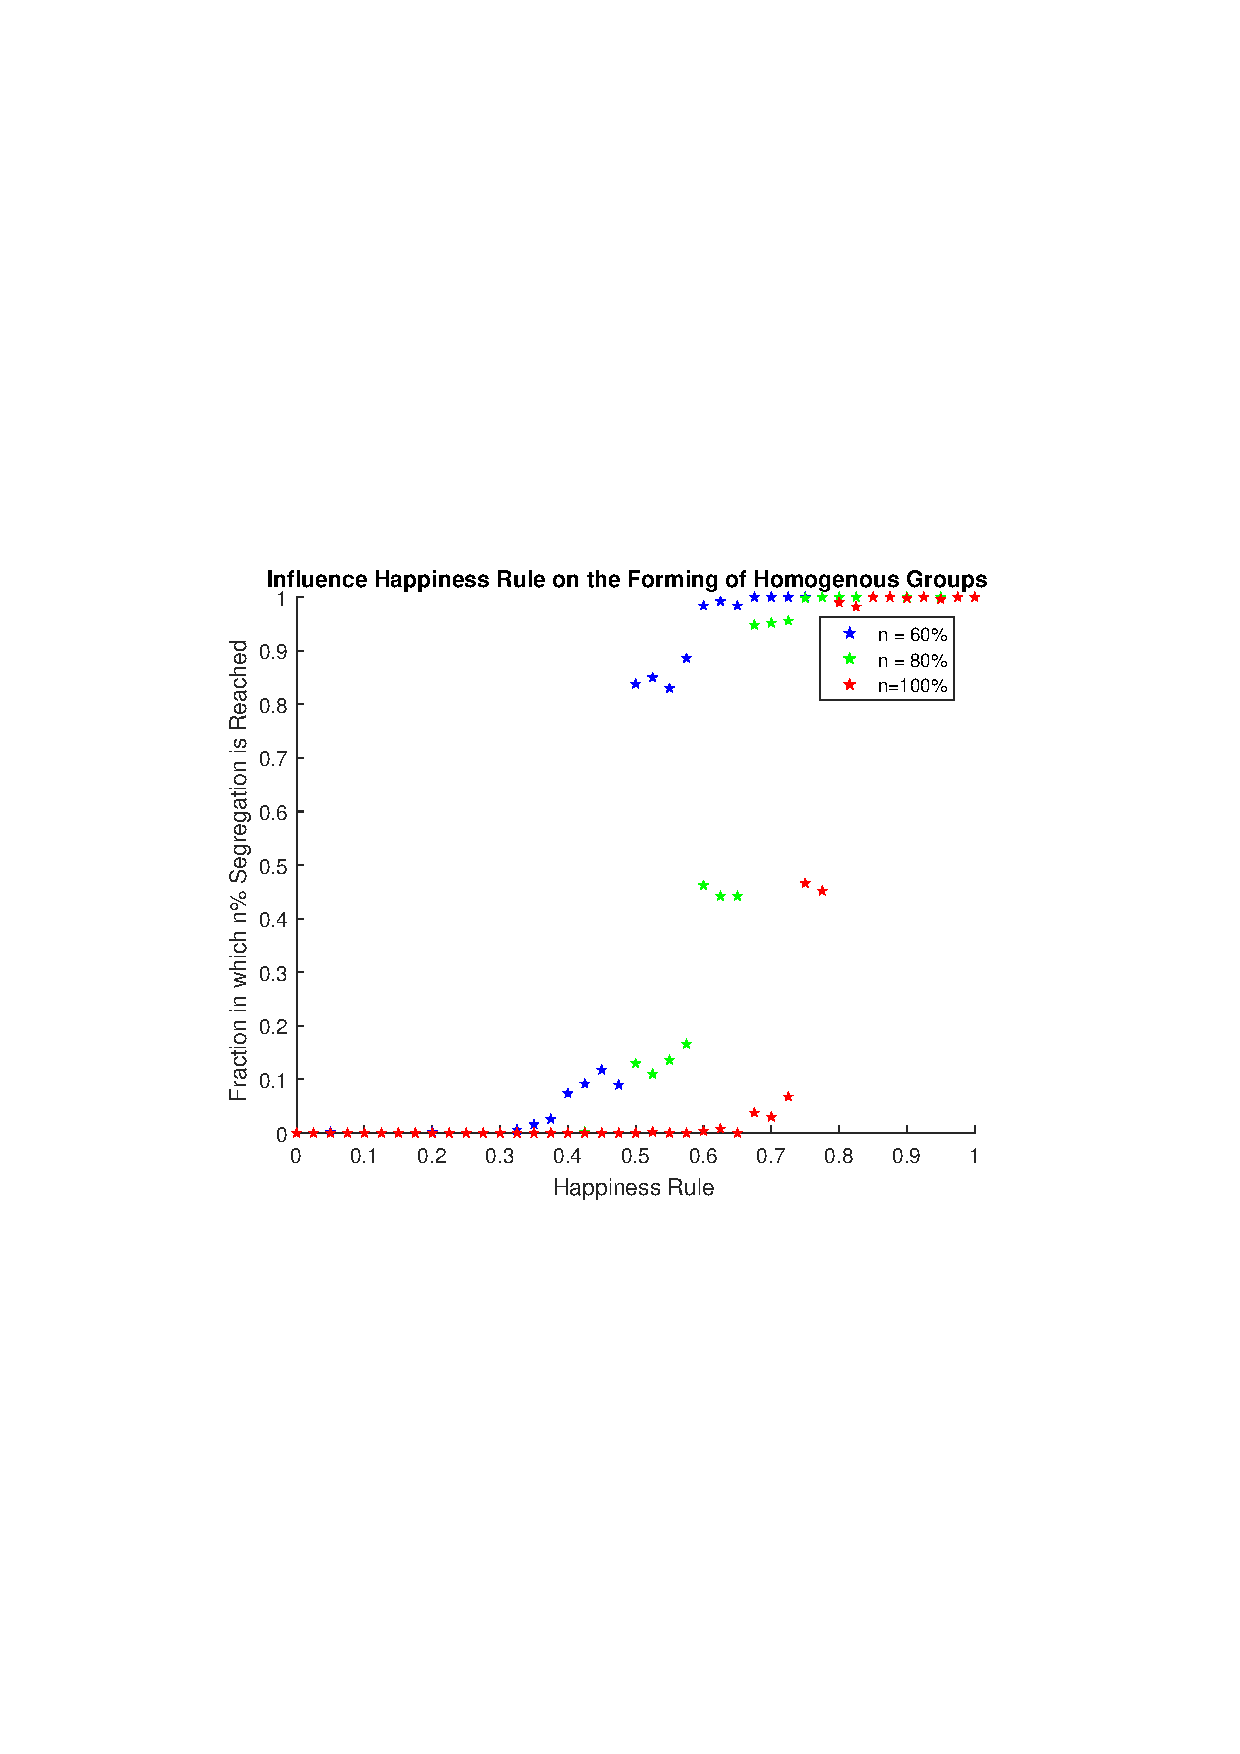
\includegraphics[width=280px]{happy_segr_60_80_100.pdf}
    \caption{For each $HR = 0,0.025,...,1$, the fraction of the simulations in which 60$\%$ (blue),80$\%$ (green) and 100$\%$ (red) segregation is reached.}
    \label{fig:happyseg4c}
\end{figure}

\subsubsection{Question 4}
We will now focus on a more relevant question, namely the distribution of the $60\%$ and $80\%$ segregation time. 
The plots are shown below.\\
To test whether the average generations $\mu_{60\%}$ it takes to reach 60\% homogenous group is equal to the average generations $\mu_{80\%}$ for 80\%. We performed the ttest2 on these two averages. The null-hypothesis is $H_0:\mu_{60\%}=\mu_{80\%}$, and $H_1: \mu_{60\%}\neq \mu_{80\%}$. For this test, we estimated $\mu_{60\%}$ and $\mu_{80\%}$ with the sample means of sample size 5000. The results are shown in tabel 2.
\begin{table}[htp]
\centering
\caption{Sample means of number of generations until 60\% and 80\% homogenous group is reached with HR 1.}
\begin{tabular}{|l|l|l|}
\hline
 Fraction homogenous group(\%)&60&80 \\ \hline
 Sample Mean&2.0892&2.8322  \\ \hline 
\end{tabular}
\end{table}
The test has rejected the null-hypothesis, which is expected because the difference of the sample means are around 0.8, which should exceeds the critical value of the test.



